\section{[Halted] The Universal Base}

The aim for this project was to create an all-purpose, powerful chassis that is lighter, simpler, and more maintainable than previous designs; Doing this would allow us to very quickly switch from competition to competition without re-building the entire robot from scratch, as well fix the robot easily.

\textit{[Halted]: Encoders can't be tested properly; Waiting for classroom return.}

\begin{figure}[h]
    \centering
    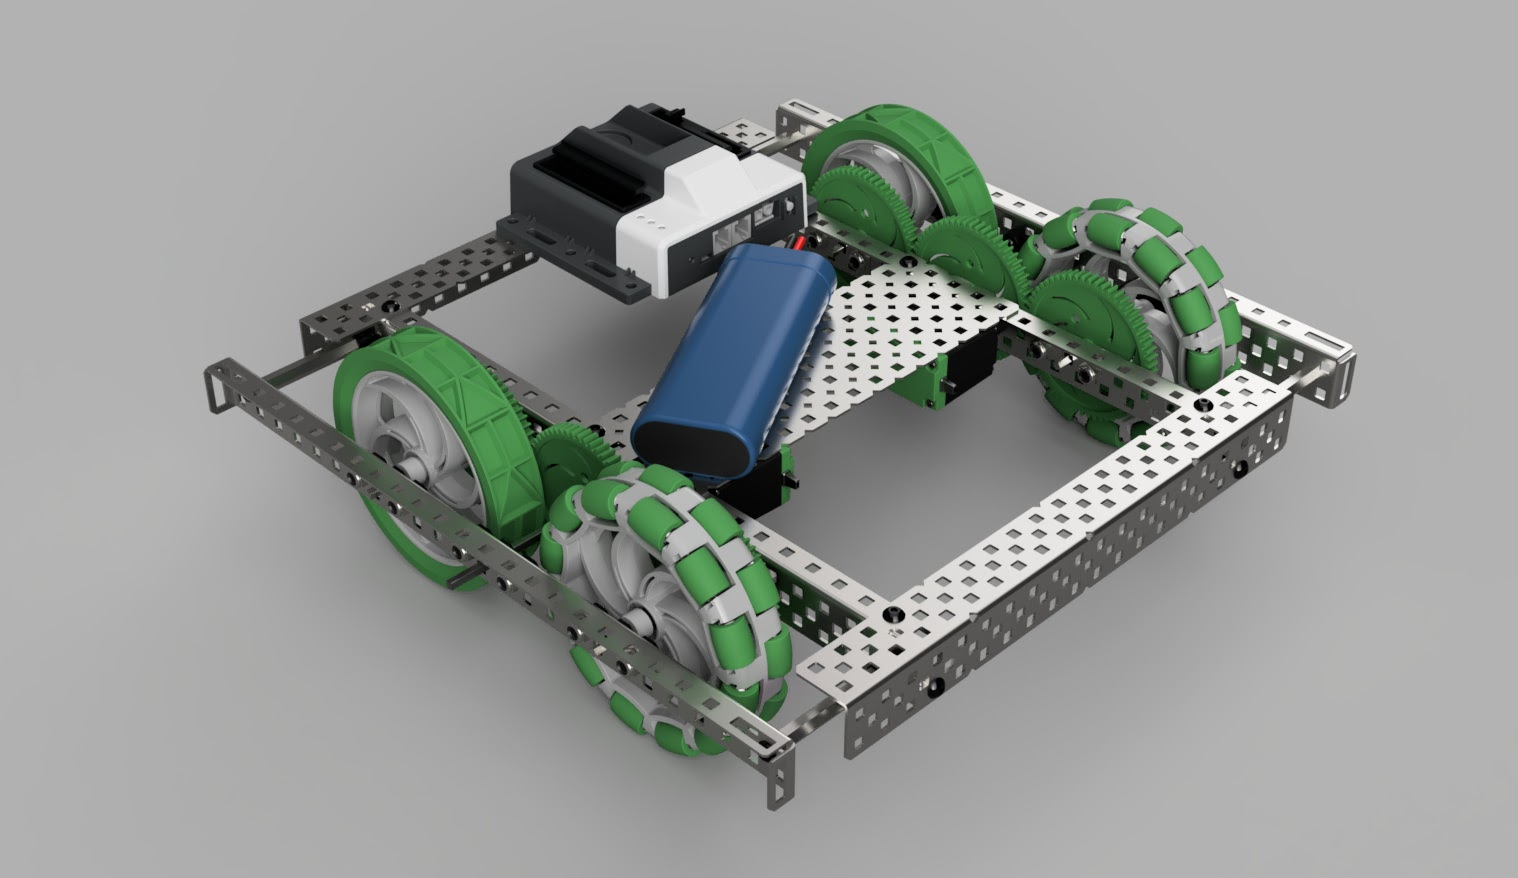
\includegraphics[width=\textwidth,height=4cm,keepaspectratio=true]{CADChassis}
    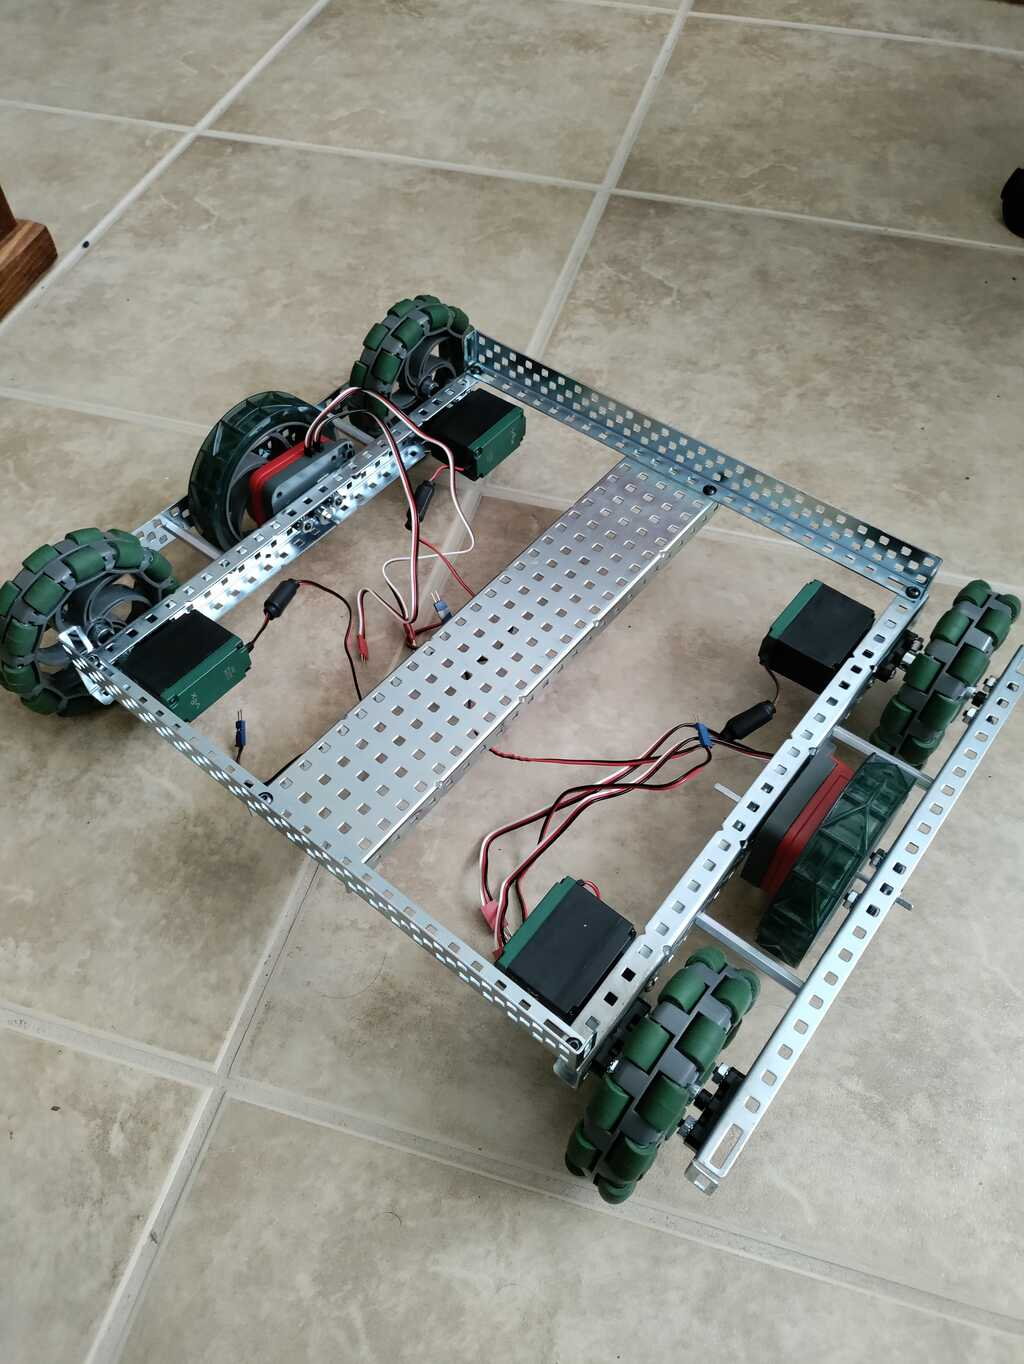
\includegraphics[width=\textwidth,height=4cm,keepaspectratio=true]{V1}
    \caption{
        (Left) An old 3D model showing a potential chassis supported by standoffs. (Right) Prototype of the proposed design using the same principle, but with 4 motors, 6 wheels, and an encoder.
    }
\end{figure}

The idea was to switch over to a 4-motor chassis that had its axes supported on both sides via standoffs; Standoffs were chosen due to requiring less metal, being easier to tighten, and allowing for a flexible chassis width. A 4-motor design was chosen due to requiring less moving parts as well as having more torque. However, in addition to 4 individually powered wheels, two unpowered wheels were going to be added in the axis of rotation, or the center, in order to have encoders be very accurate without dealing with wheel slip.

\begin{figure}[h]
    \centering
    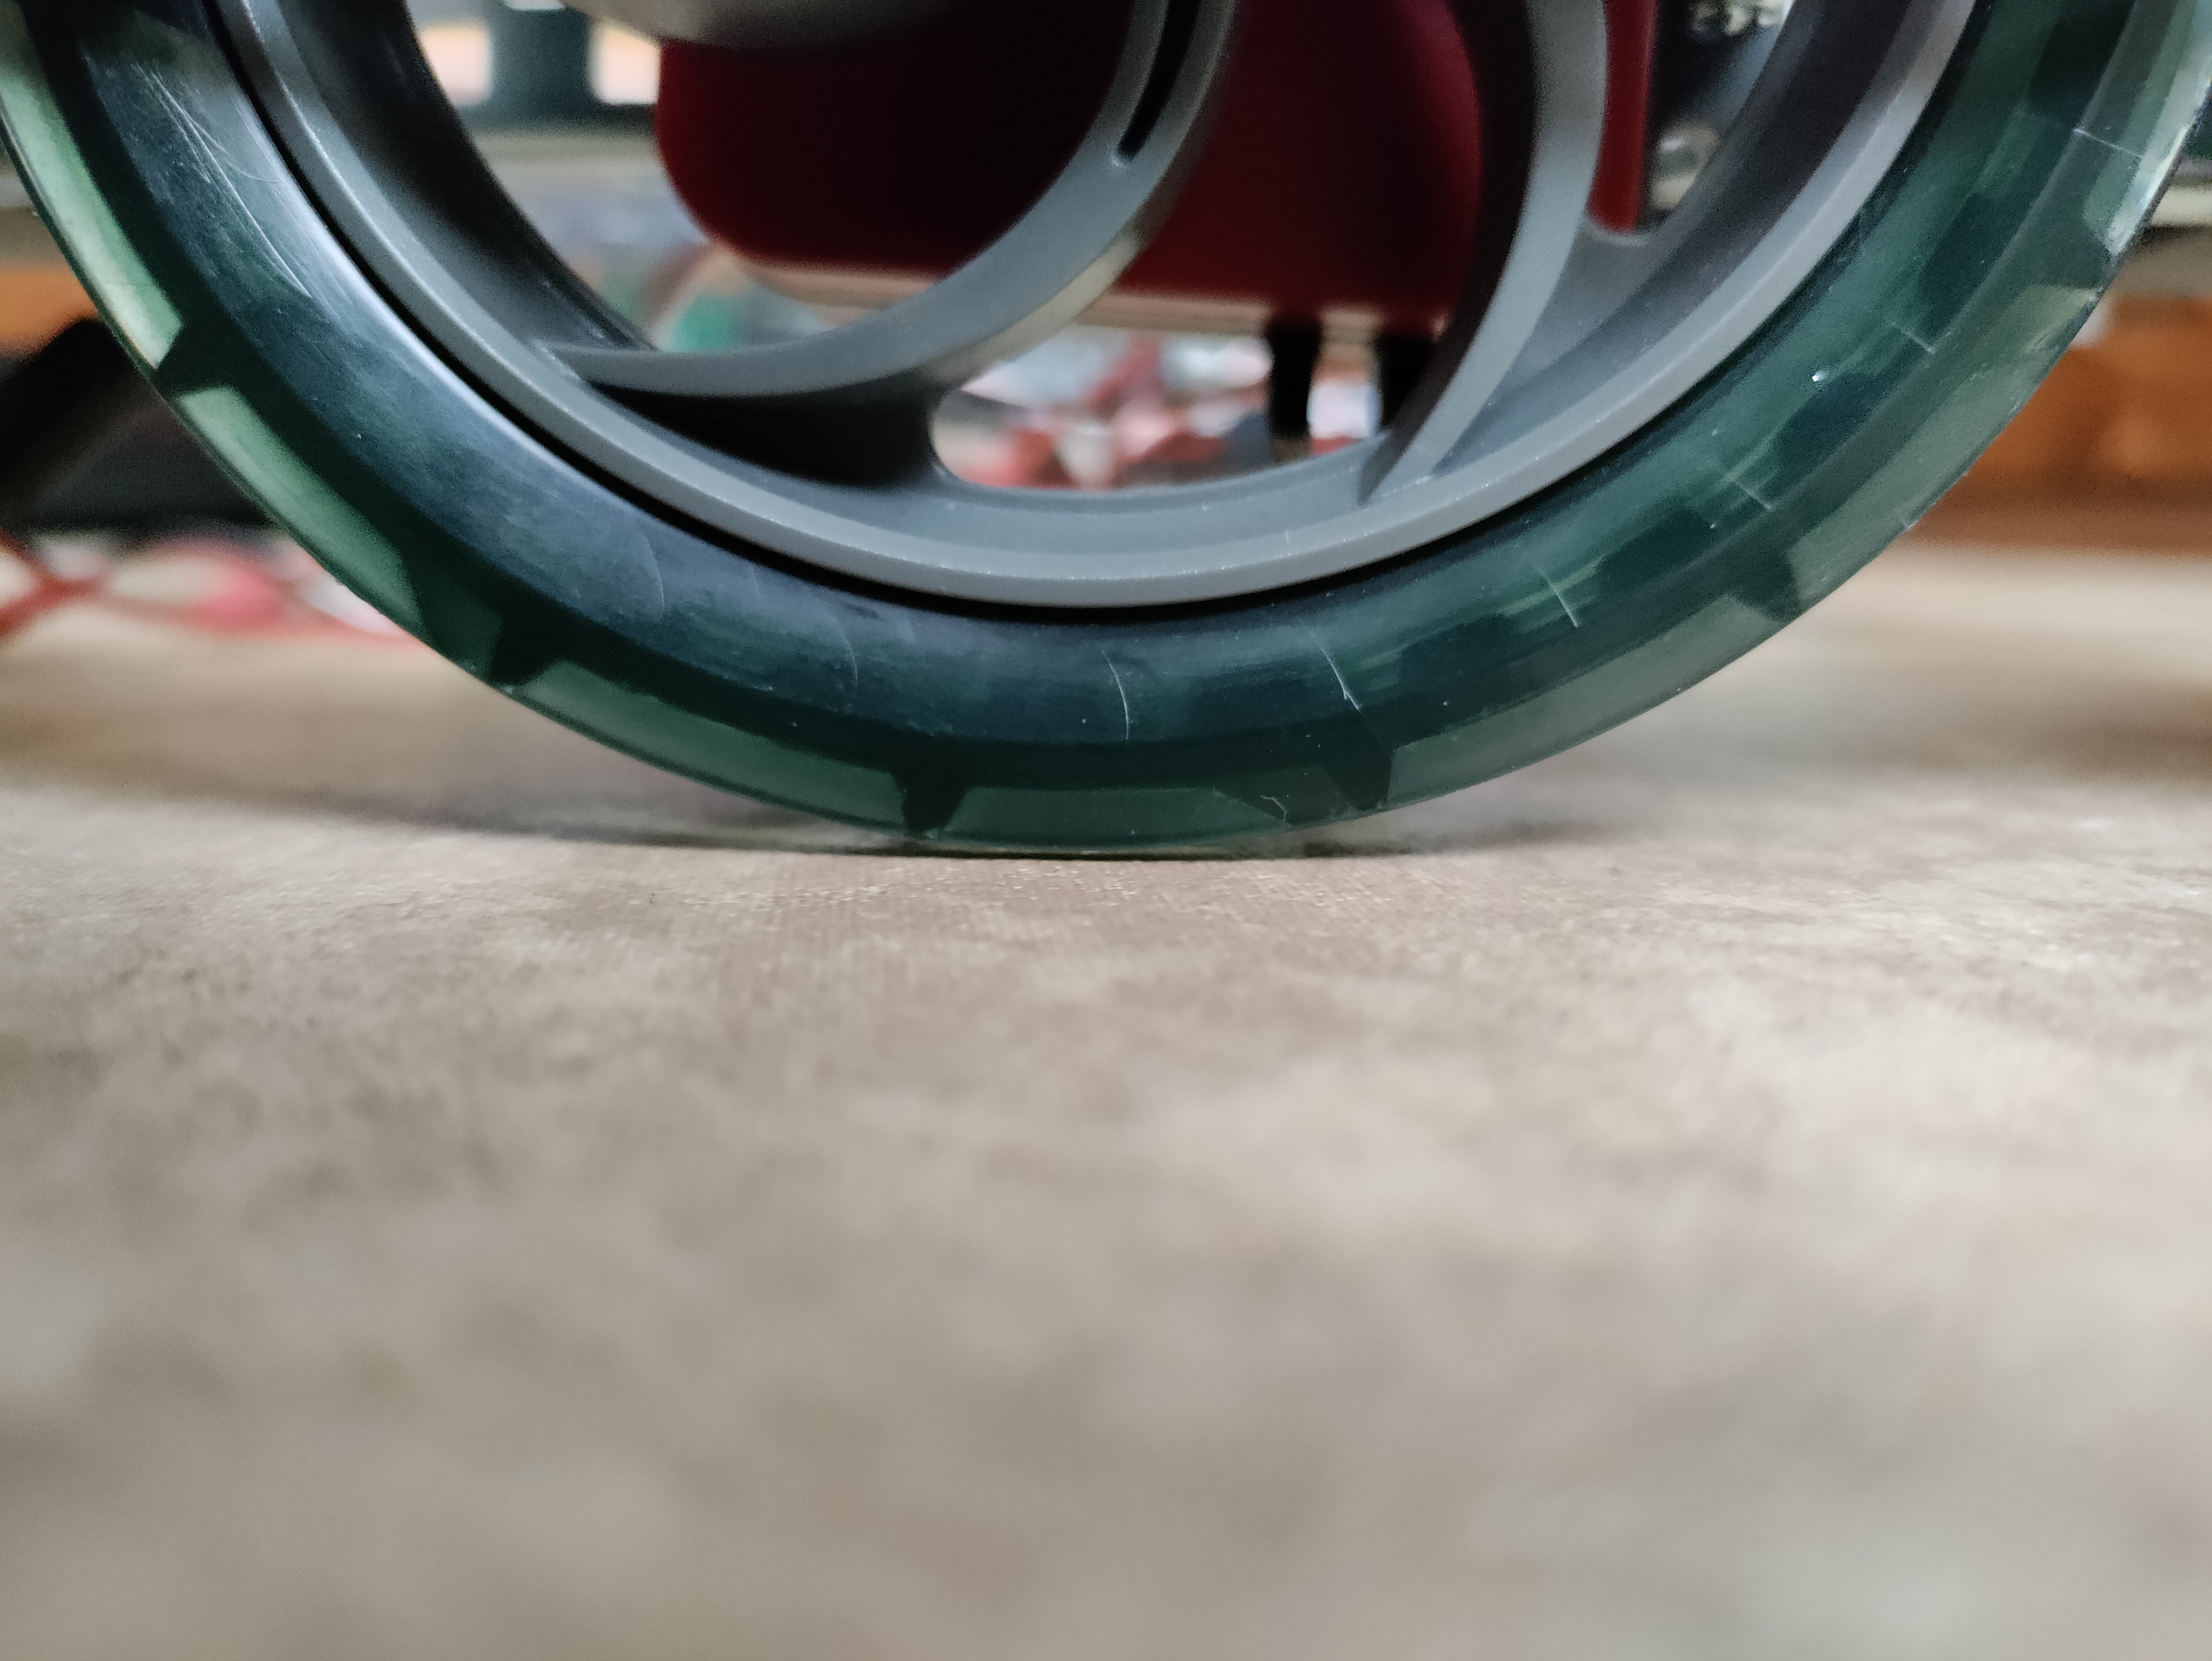
\includegraphics[width=\textwidth,height=3cm,keepaspectratio=true]{OGWheels}
    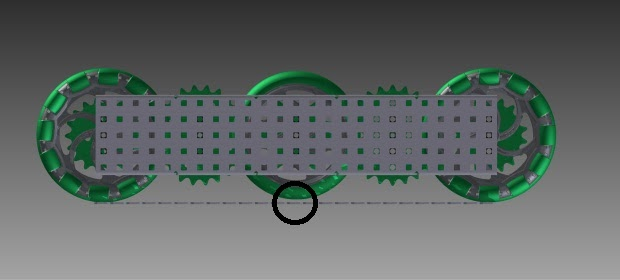
\includegraphics[width=\textwidth,height=3cm,keepaspectratio=true]{CADWheels}
    \caption{
        (Left) The prototype's wheel being ~500 microns off a tiled floor. (Right) A 3D model showing that the difference in size is caused by the wheels themselves, not any external factor.
    }
\end{figure}

Upon building the chassis, it was apparent that the unpowered encoder wheels were not touching the ground. Via a 3D model, I found out that holonomic wheels were a millimeter bigger in diameter. While this may not be a problem in carpet or foam environments where the floor has some give, my smooth tile floor made it near impossible for the two traction wheels to gain any traction. I did not give up, and slapped rubber bands and duct tape on the wheels to make up for that gap.

\begin{figure}[h]
    \centering
    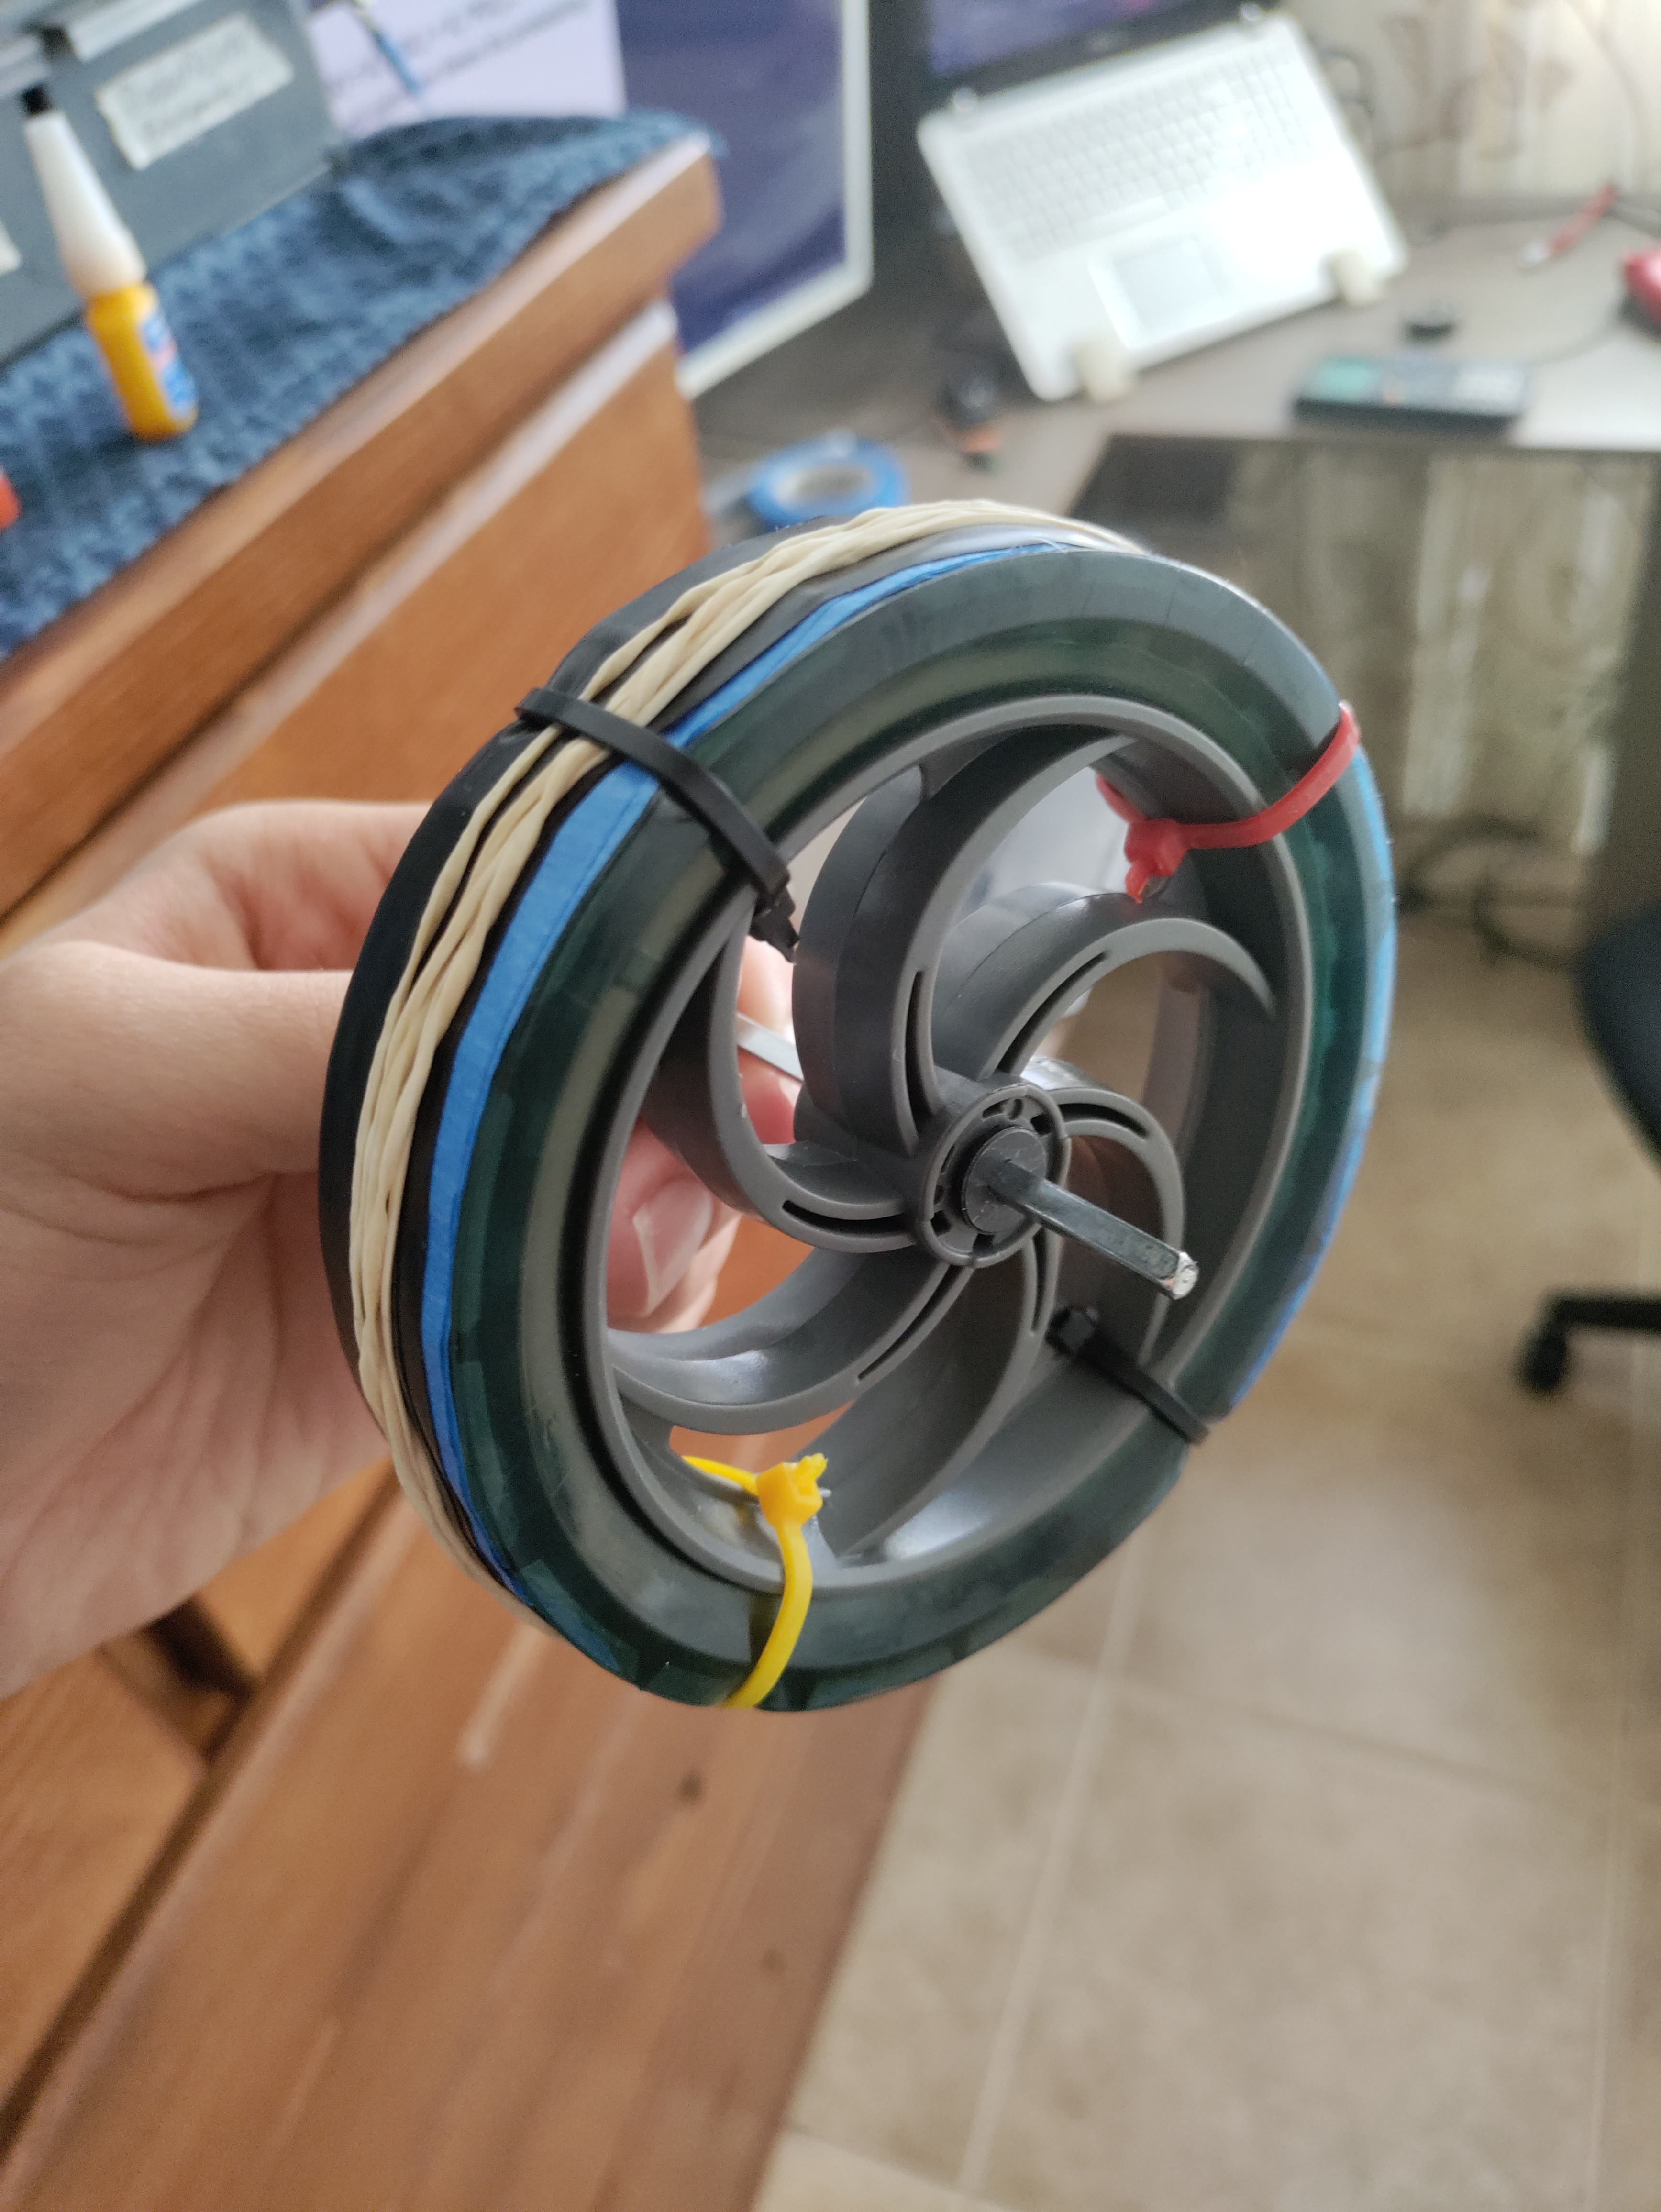
\includegraphics[width=\textwidth,height=6cm,keepaspectratio=true]{SuperWheel}
    \caption{
        A super wheel.
    }
\end{figure}

I went through various iterations of layering to fix this issue. Blue tape, blue tape + rubber bands, blue tape + electrical tape, blue tape + electrical tape + rubber bands, all with varying amounts of tape and rubber bands. Fortunately, the blue tape + electrical tape + rubber band wheel, or "super wheel", worked excellently and consisted of 5 layers of duct tape, 2 layers of electrical tape, and 5 rubber bands. Unfortunately, my tiled floor had spaced valleys that momentarily lifted a wheel or two off the ground when driving, making a good test with an encoder very difficult.

With the prototype showing somewhat promising results in every other department, I rebuilt the robot in a way where it's very maintainable. Mainly, I flipped the side metal bars so that the shaft collars holding the wheels together are exposed, so that you can easily remove and attach the wheels in case anything goes wrong. I also made extra sure all screws holding the robot together were screwed outside to in, making it very easy to tighten nearly all parts of the robot without awkwardly tightening it from the inside.

All in all, the chassis is incredibly study, has very customizable chassis width and length to make sensor and arm mounting a lot easier, and a lot more maintainable (from experience). The maximum size of the robot is 18" x 15.5" if it were built with the same parts I used, or 17" x 15.5" if we take very special care building it. If for any reason the building constraints shrink, we can swap the X-axis and Y-axis bars with 15-hole C-channel, ditch the encoder wheels, and get the smallest possible size of 13" x 10".

\textit{Note:} This base needs further testing in the classroom to determine if the encoders are actually accurate.

\subsection{The Process}
Here are some pictures I took while solving the tiny-gap issue.

\begin{figure}[h]
    \centering
    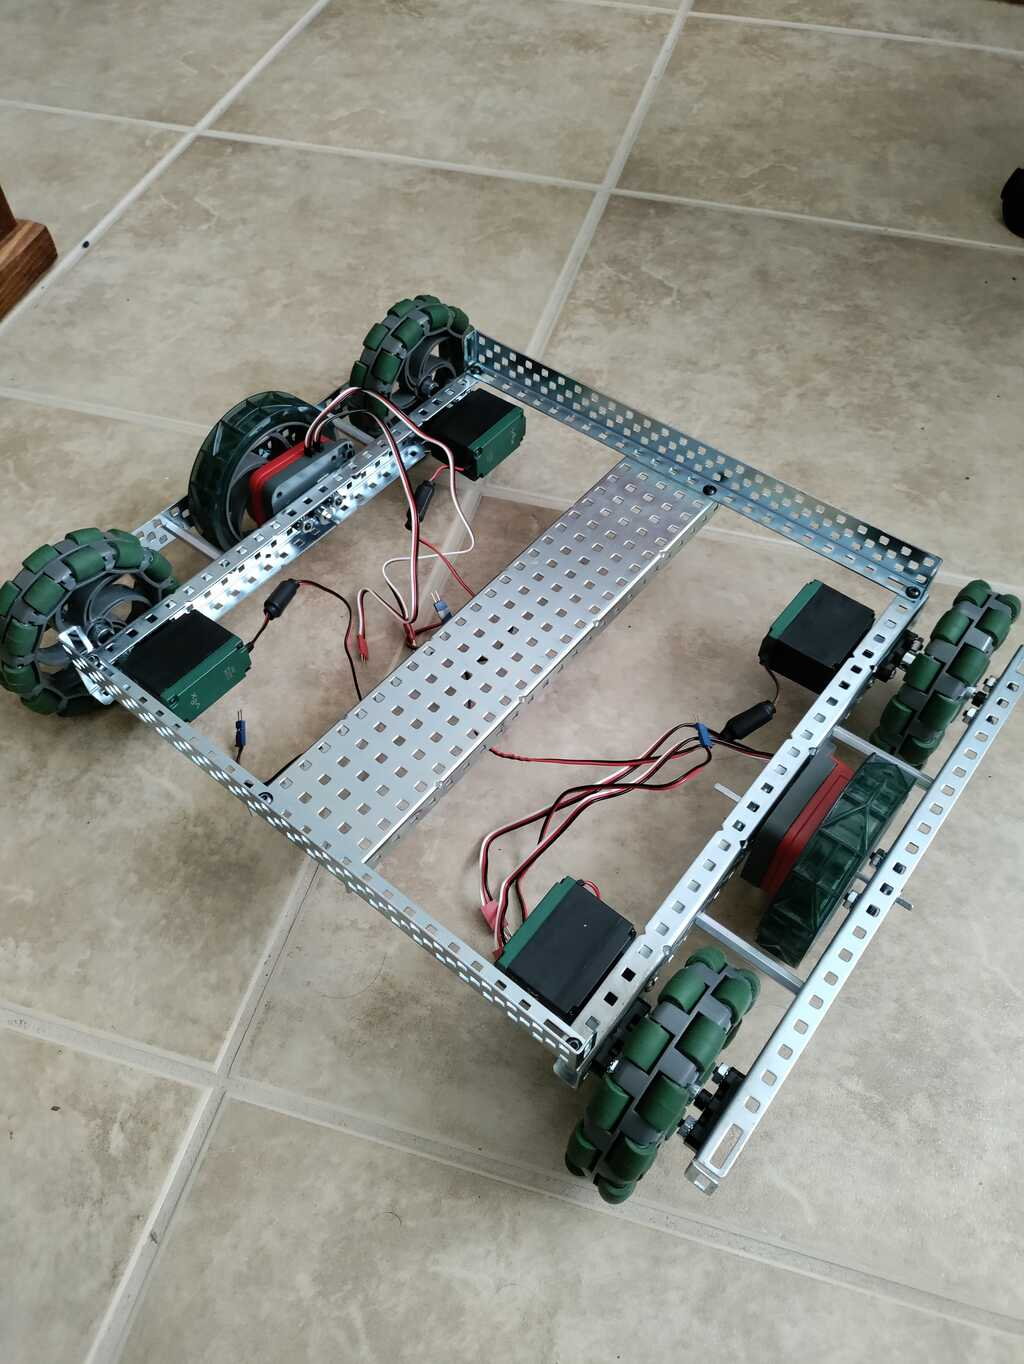
\includegraphics[width=\textwidth,height=5cm,keepaspectratio=true]{V1}
    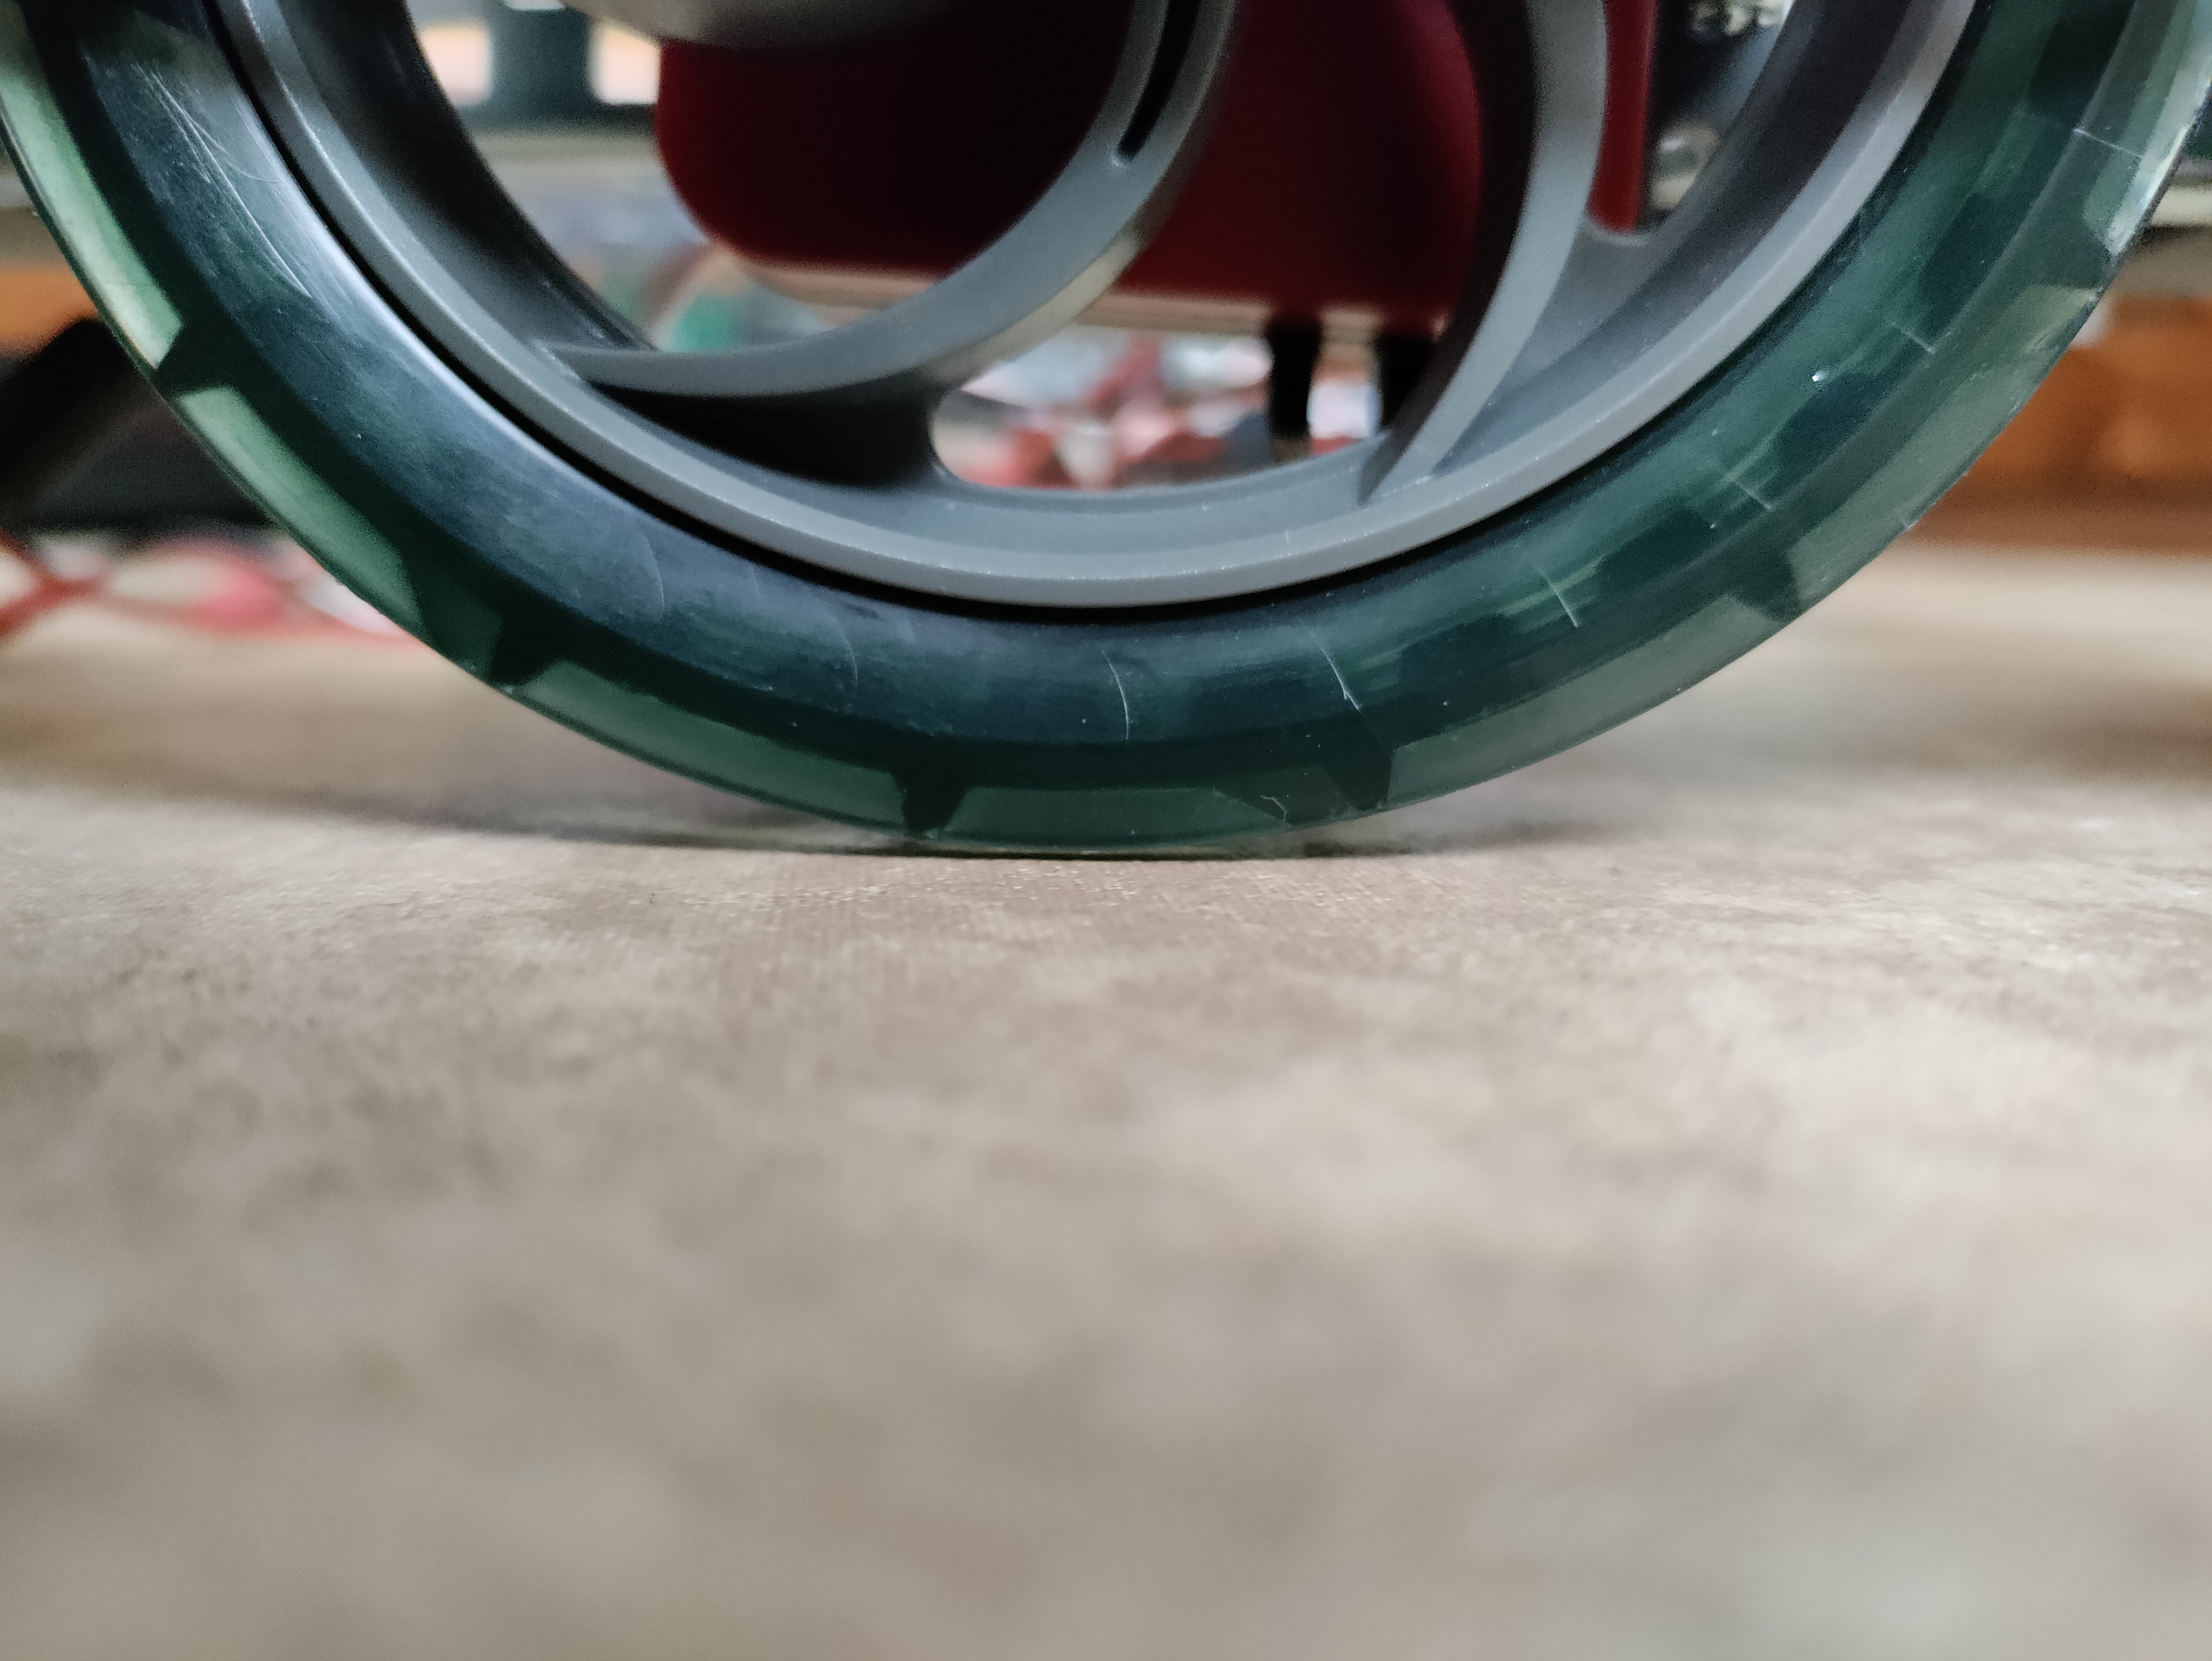
\includegraphics[width=\textwidth,height=5cm,keepaspectratio=true]{OGWheels}
    \caption{
        Where the issue presented itself.
    }
\end{figure}

\begin{figure}[h]
    \centering
    \includegraphics[width=\textwidth,height=5cm,keepaspectratio=true]{V2Front}
    \includegraphics[width=\textwidth,height=5cm,keepaspectratio=true]{V2Side}
    \caption{
        I first added multiple layers blue tape before adding rubber bands. The wheel made contact just fine, but it was slippery, lifted other wheels up, and jammed itself when the rubber band came loose.
    }
\end{figure}

\begin{figure}[h]
    \centering
    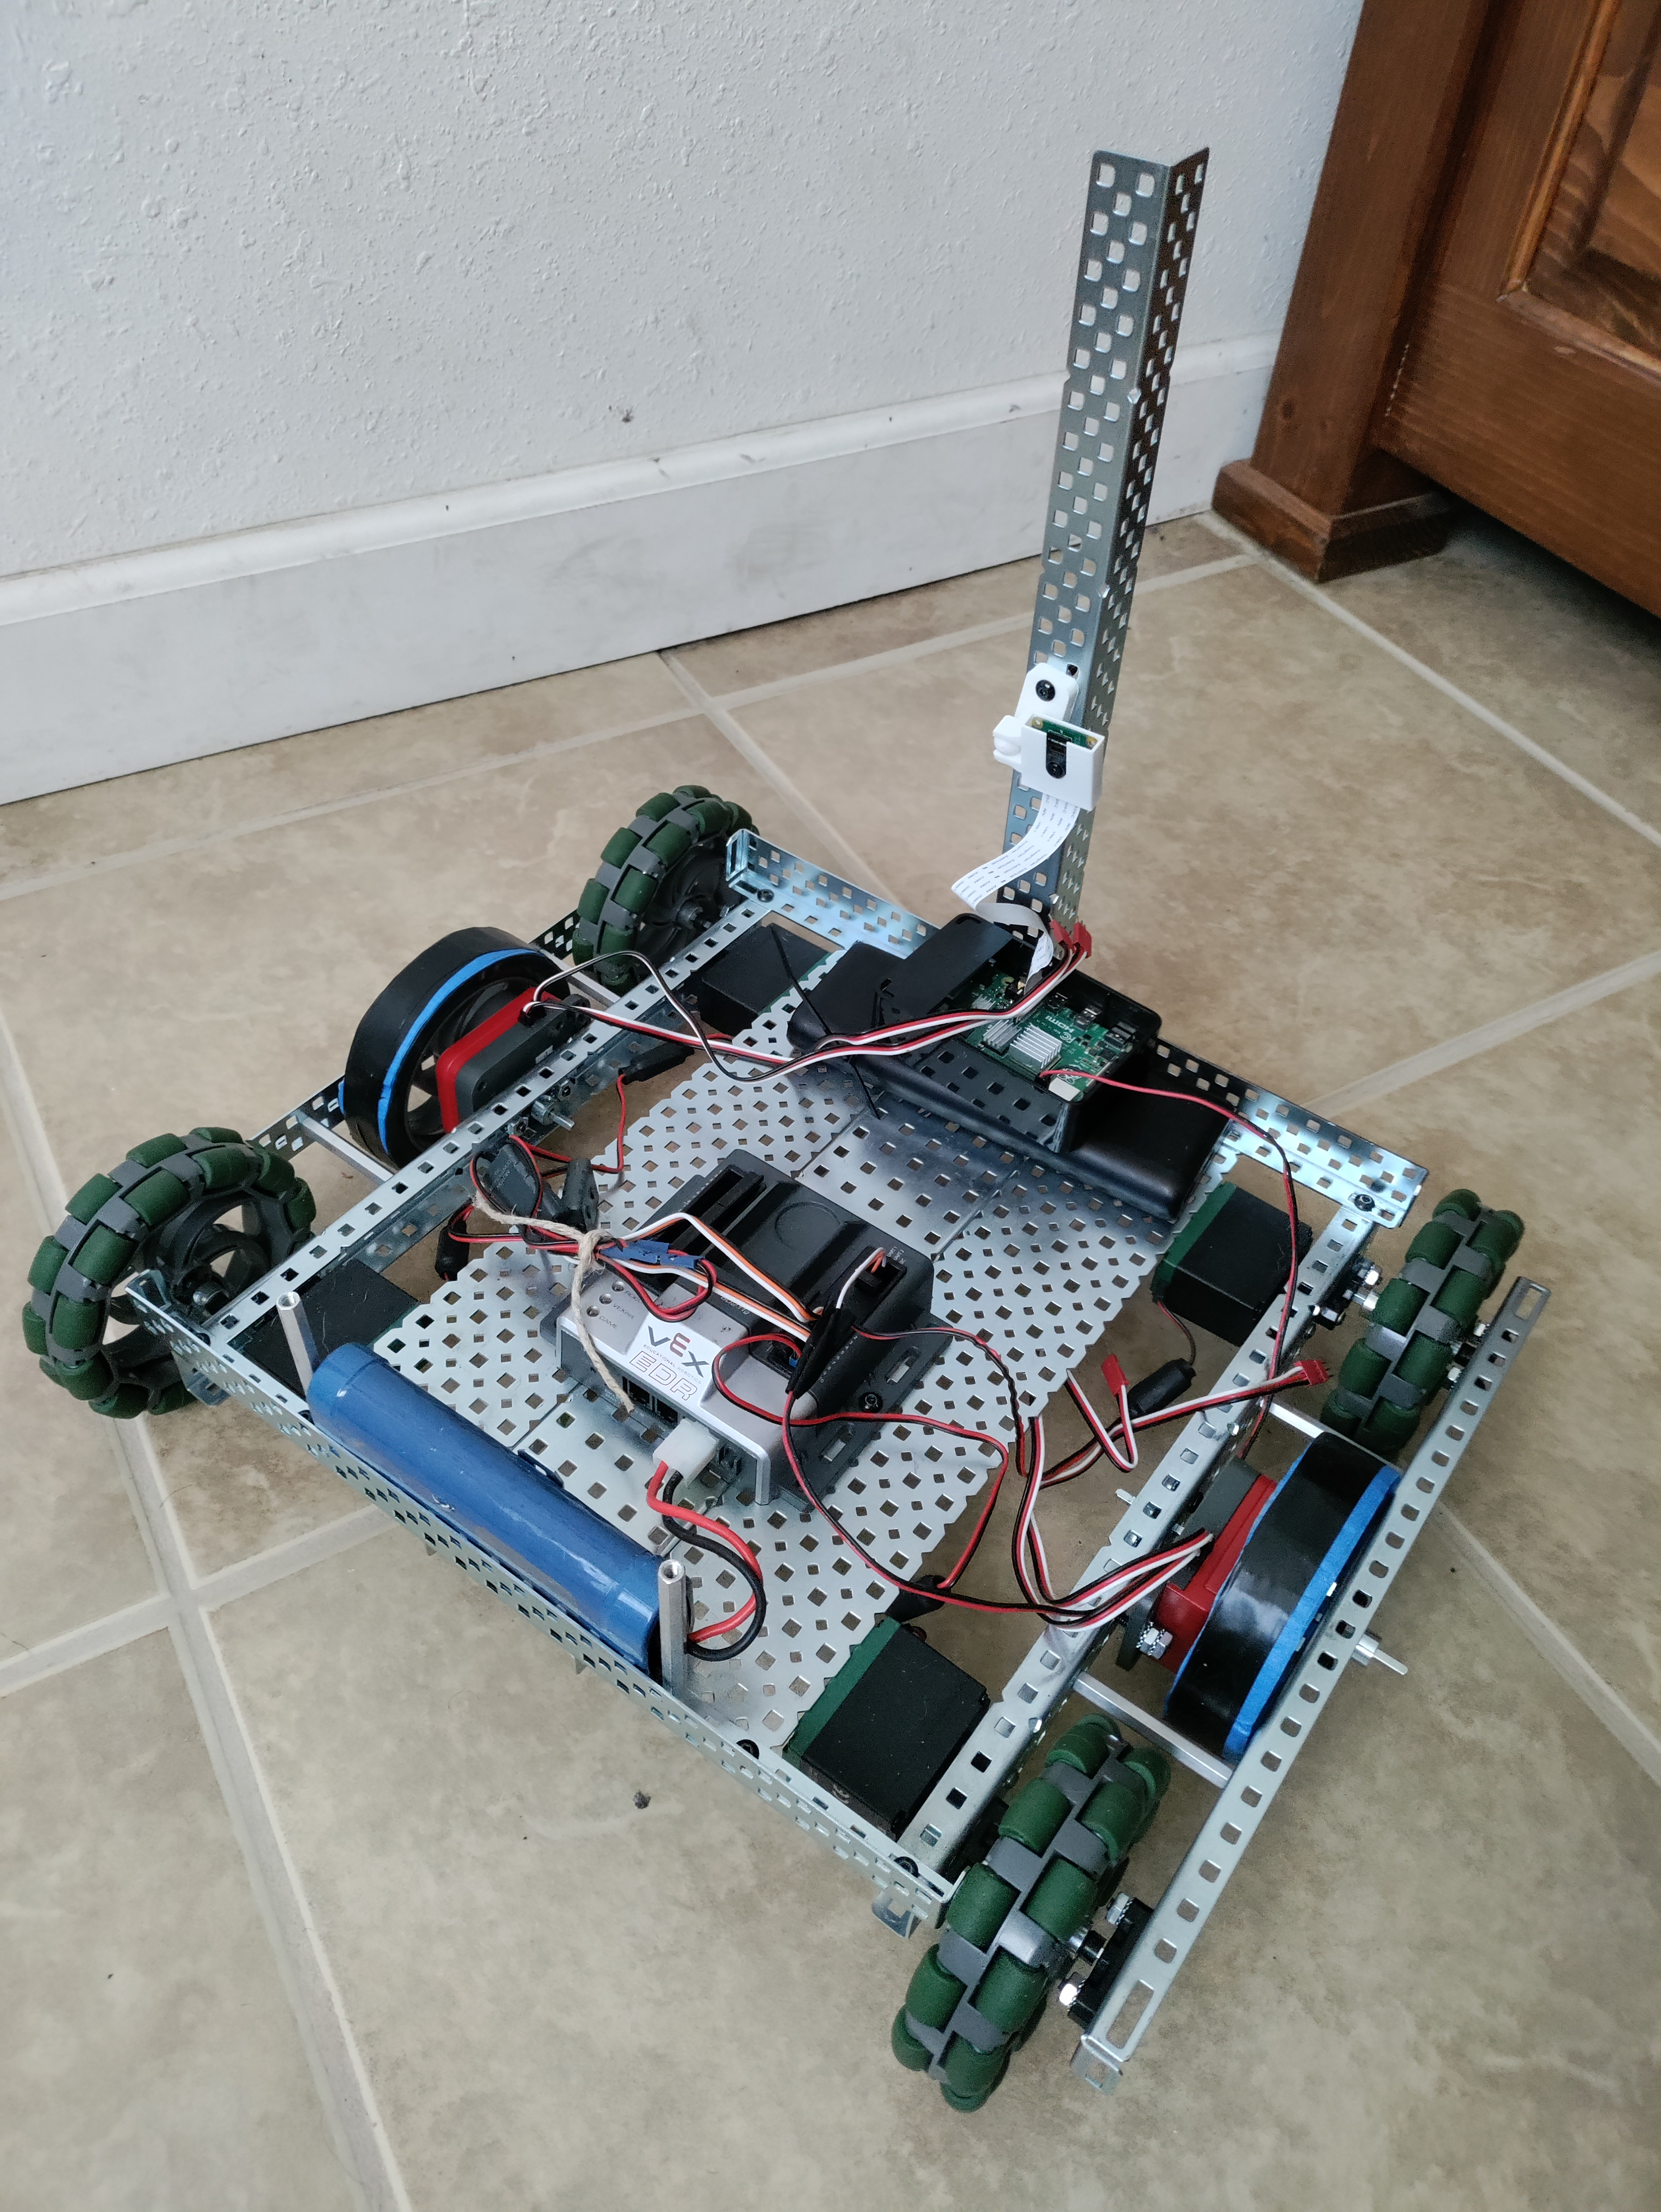
\includegraphics[width=\textwidth,height=6cm,keepaspectratio=true]{V4}
    \caption{
        Eventually, I put electrical tape on top of blue tape as it had more traction with the ground. It worked a lot better, but it still slipped.
    }
\end{figure}

\begin{figure}[h]
    \centering
    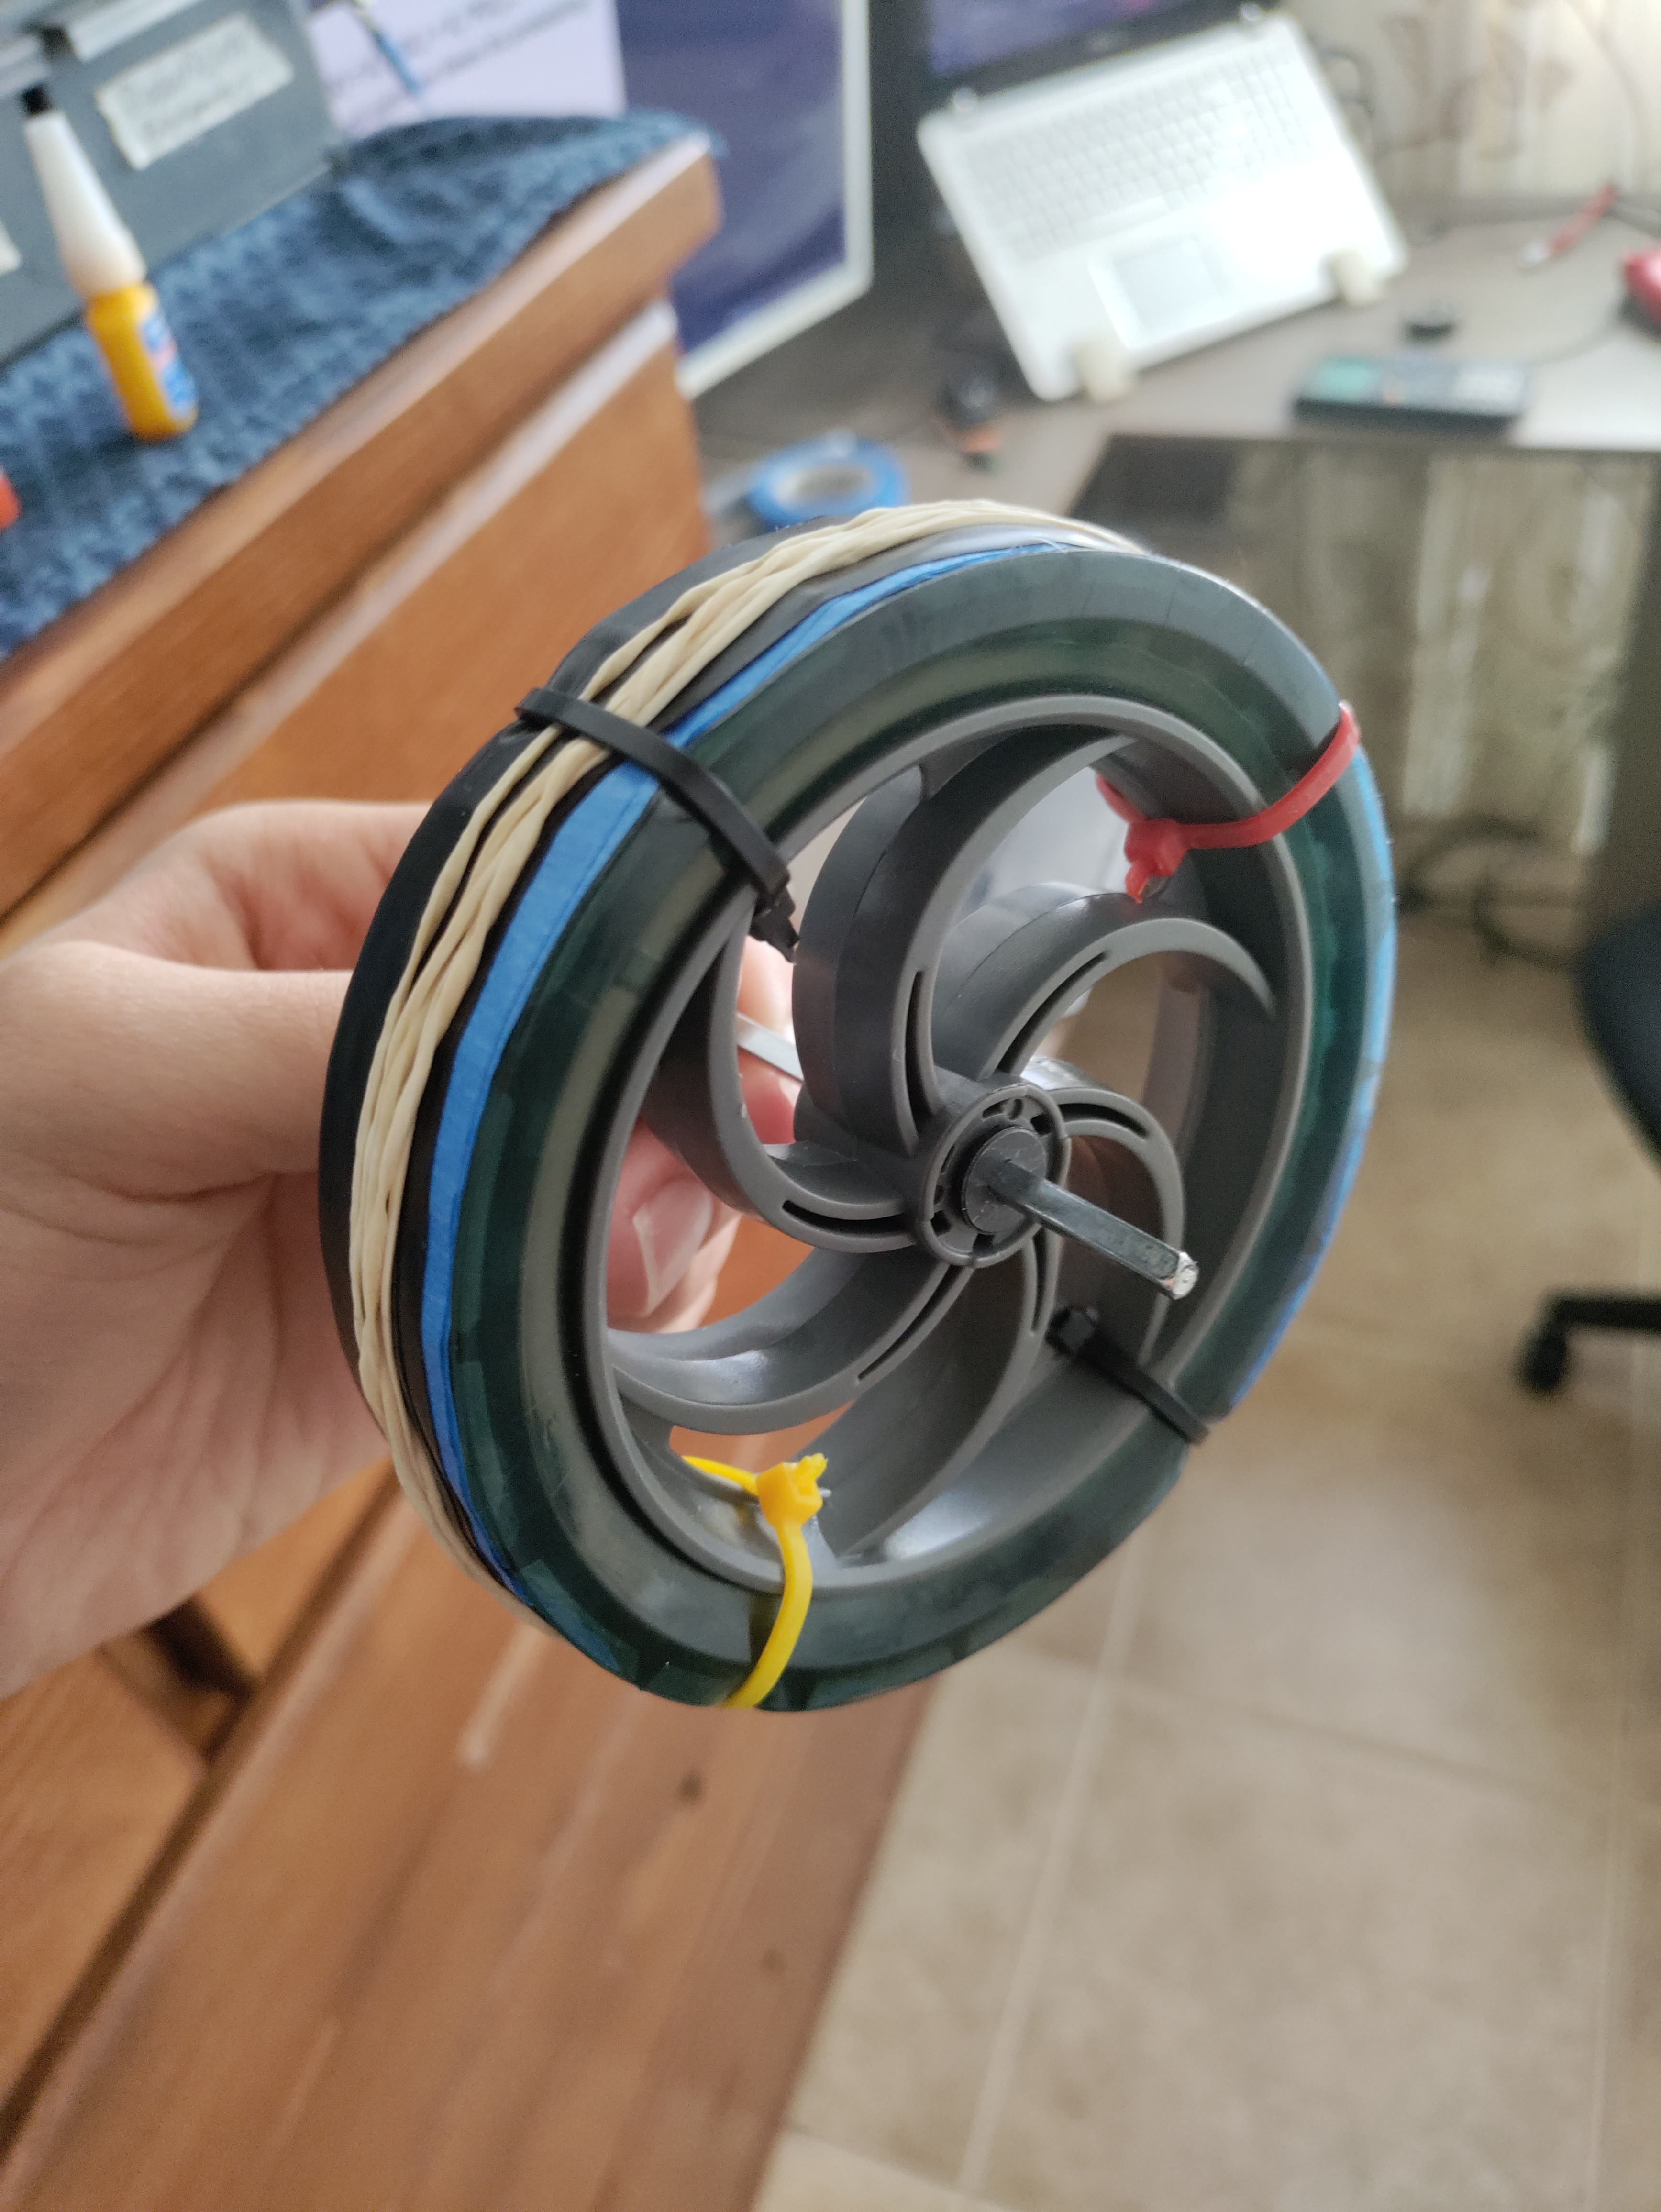
\includegraphics[width=\textwidth,height=4cm,keepaspectratio=true]{SuperWheel}
    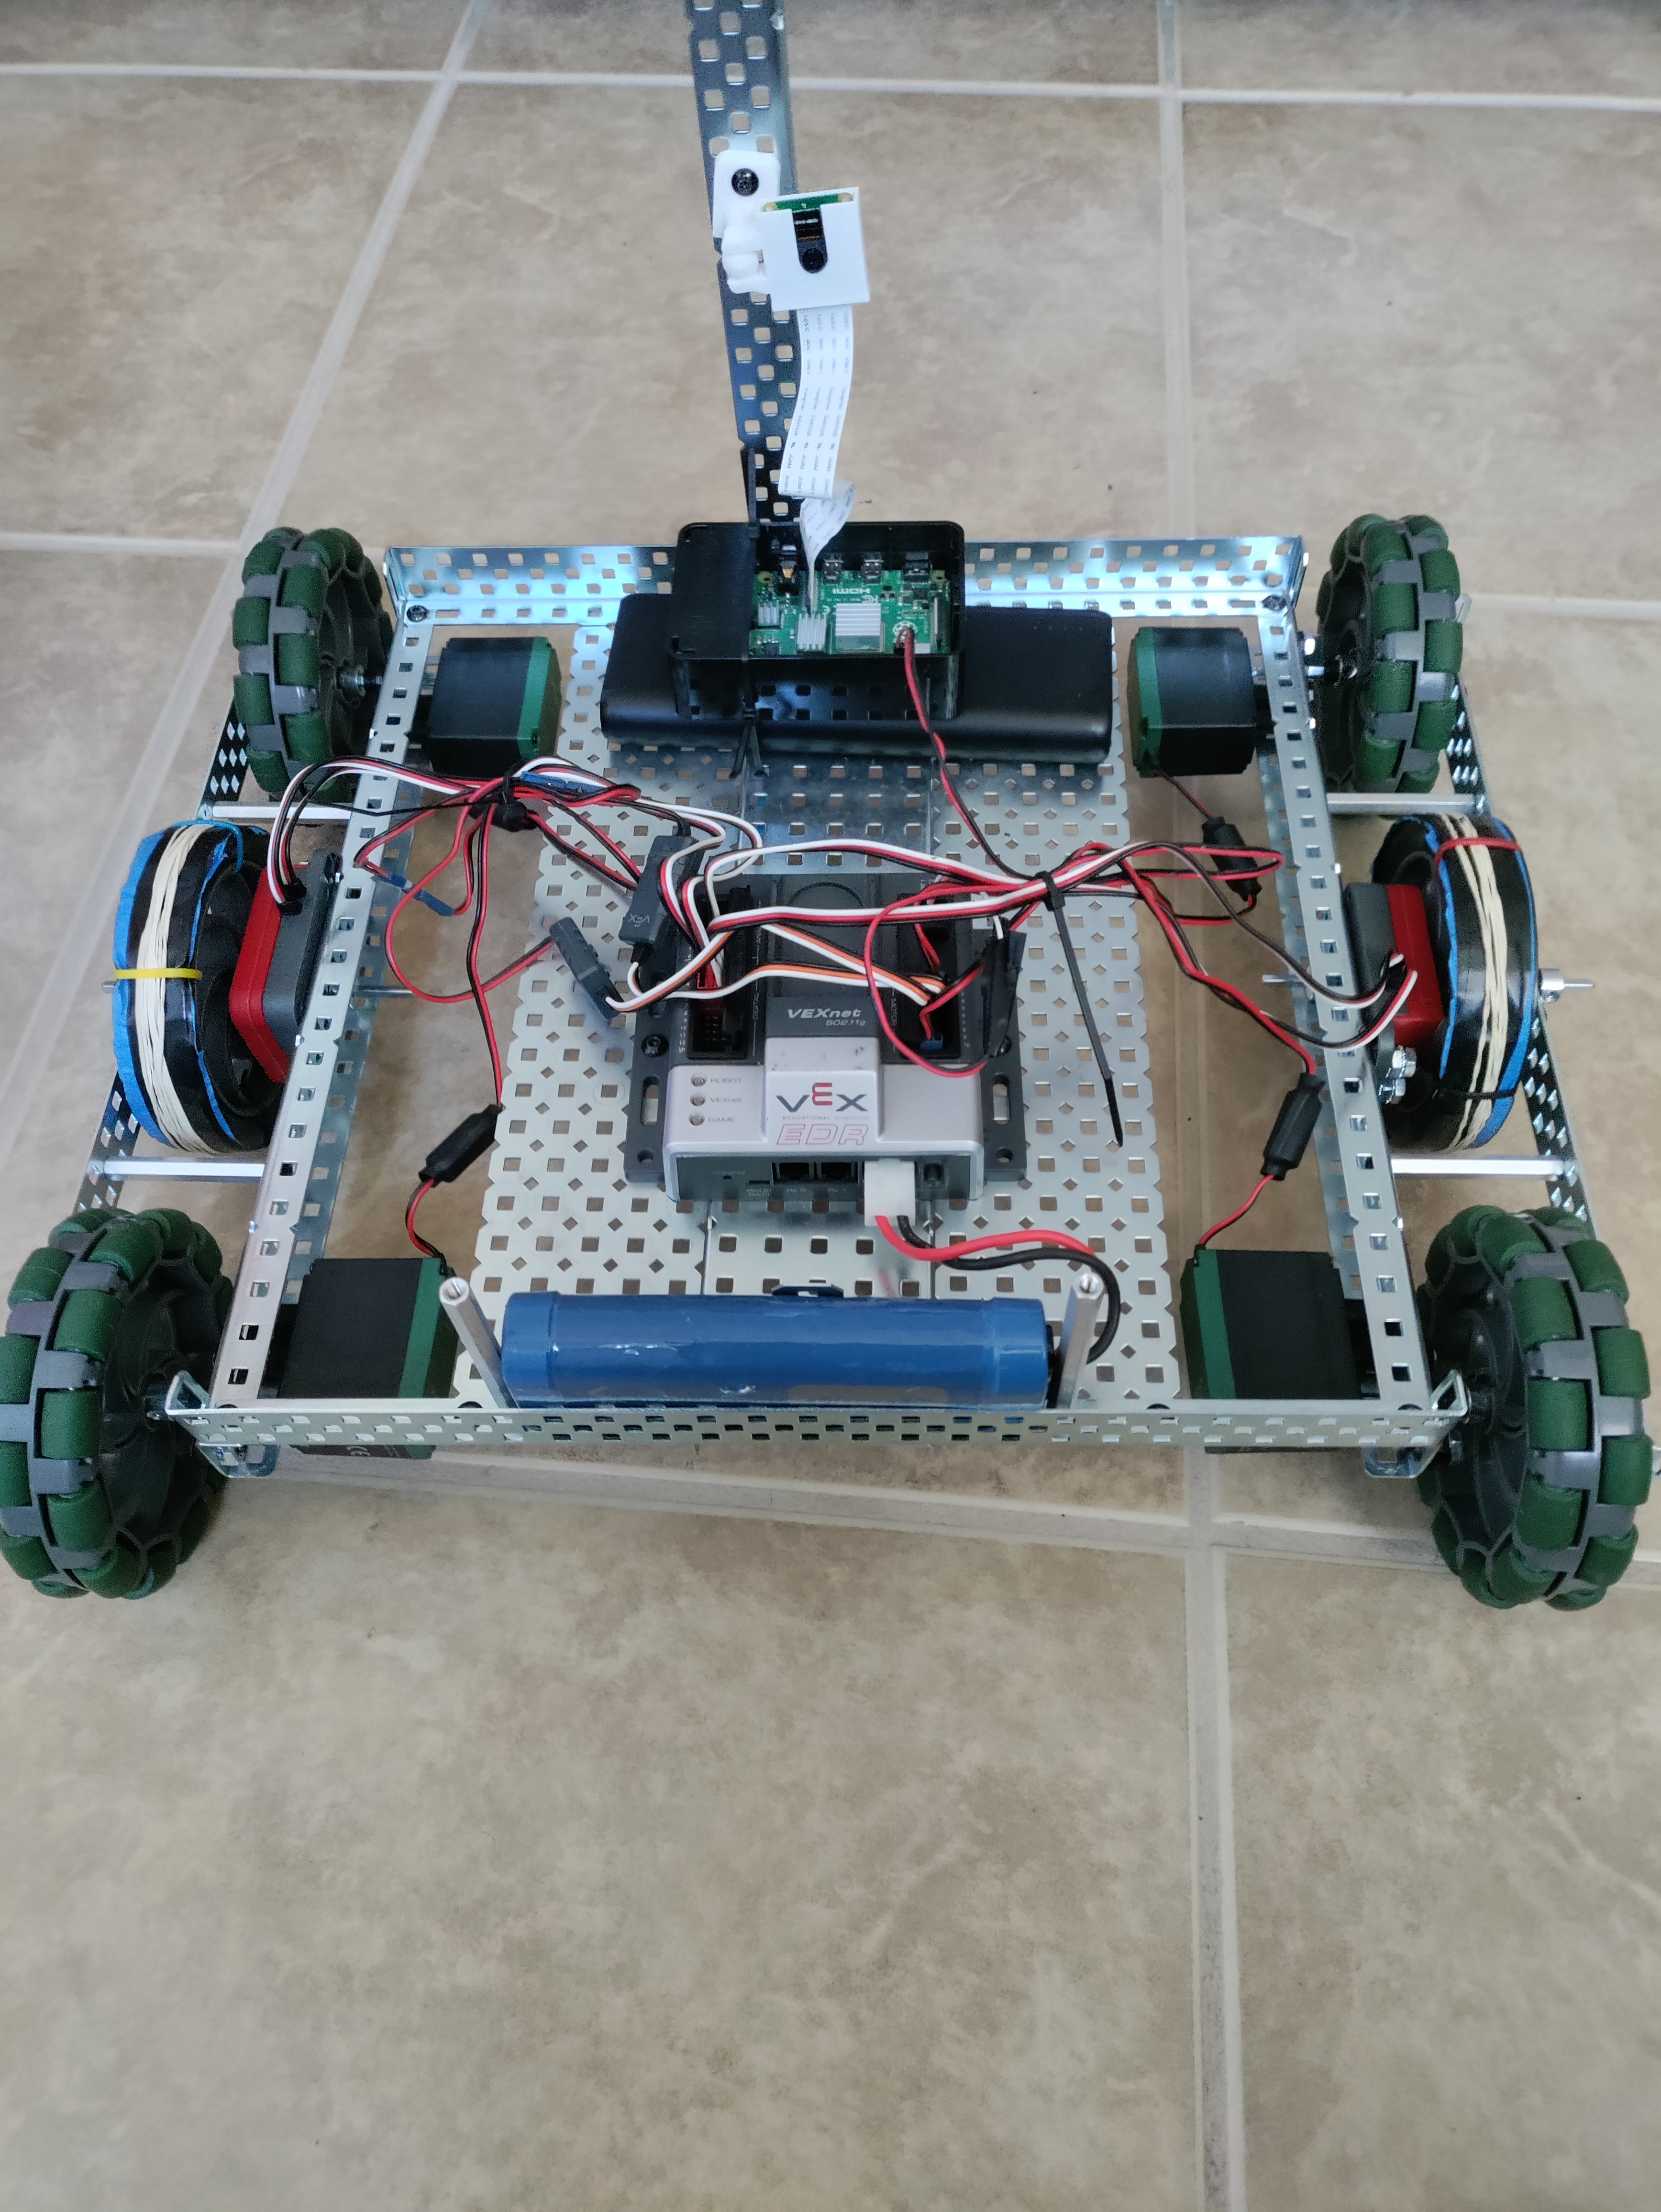
\includegraphics[width=\textwidth,height=4cm,keepaspectratio=true]{V5Front}
    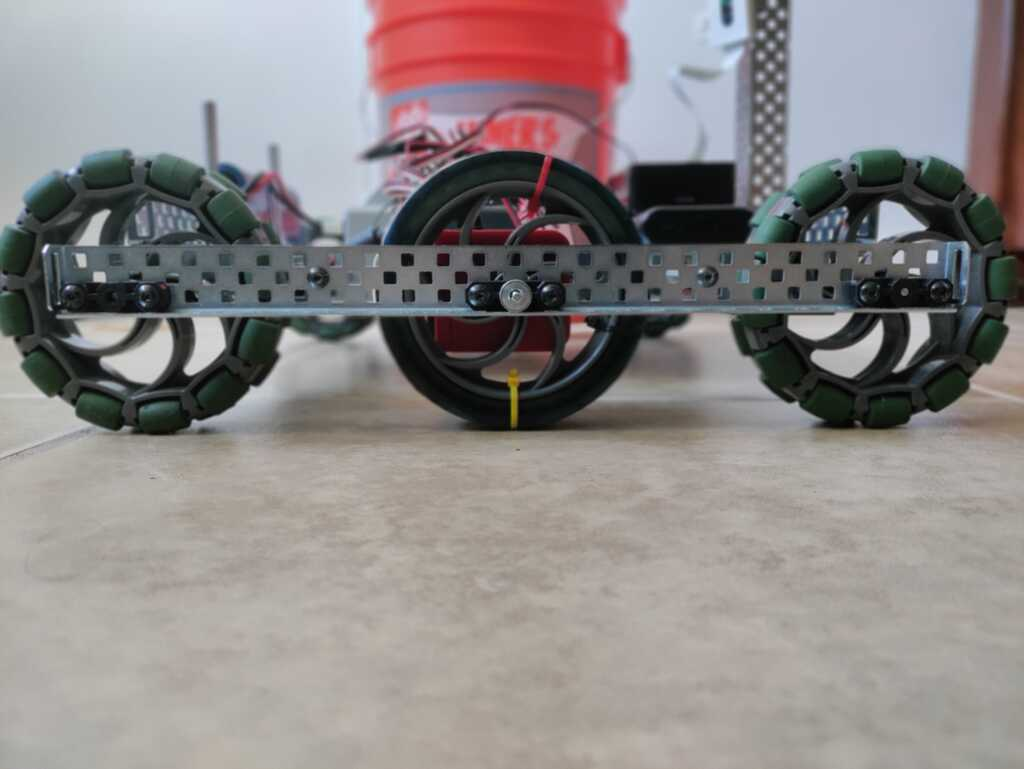
\includegraphics[width=\textwidth,height=4cm,keepaspectratio=true]{V5Side}
    \caption{
        Here I put the super wheels and it worked perfectly. Unfortunately, a wheel always lifted off the ground when driving across the valleys in my floor.
    }
\end{figure}


\begin{figure}[h]
    \centering
    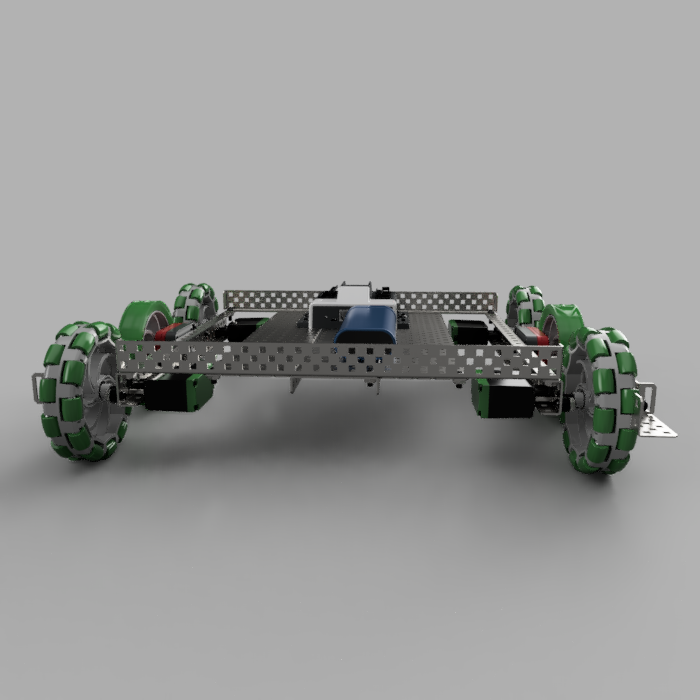
\includegraphics[width=\textwidth,height=7cm,keepaspectratio=true]{V5CAD}
    \caption{
        I preserved it as a CAD for the future.
    }
\end{figure}
